\documentclass[hyperref=colorlinks]{beamer}
\mode<presentation>
\usetheme{iclpt}
\setbeamertemplate{navigation symbols}{}
\setbeamertemplate{headline}{
\begin{beamercolorbox}[leftskip=.2cm,rightskip=.2cm,topskip=.2cm,ht=1.1cm,dp=0.1cm,wd=\textwidth]{institute in head/foot}
  
\includegraphics[height=1cm]{icl.pdf}
  \hfill
  
\includegraphics[height=1cm]{../Pics/CMS-Color.pdf}
\end{beamercolorbox}
}
\setbeamertemplate{footline}{
\begin{beamercolorbox}[ht=.55cm,dp=0.4cm,wd=\textwidth,leftskip=.3cm]{author in head/foot}%
  \begin{minipage}[c]{5cm}%
    \usebeamerfont{author in head/foot}
    \insertshortauthor 
    \insertshorttitle
    \end{minipage}\hfill%
  \insertframenumber{} / \pageref{lastframe}
  \hfill
  \begin{minipage}{6cm}
    \hfill
  \end{minipage}
\end{beamercolorbox}%
}

\usepackage{color}
\usepackage{tabularx,colortbl}
\usepackage{graphicx}
\usepackage{pdfpages}
\usepackage{feynmp}
\DeclareGraphicsRule{*}{mps}{*}{}

\title{MC Jet Resolution Study}
\author[P. Dunne]{P. Dunne}
\date{}
\begin{document}
\begin{fmffile}{feynmandiags}

%TITLE PAGE
\section{Title}
\begin{frame}
  \titlepage

\end{frame}

%OUTLINE
\begin{frame}
  \frametitle{Introductinon}
    \vspace{-0.3cm}
    \vspace{-0.2cm}
    \begin{block}{}
      \footnotesize
      \begin{itemize}
      \item MC jet resolution used in smearing method for jets without a gen jet match
      \item We still have differences between analysis A \& B in the $W\rightarrow\tau\nu$ background due to smearing
      \item Analysis A use MC resolutions from Spring '10 
      \item JetMET POG recommend measuring MC resolution yourself
      \end{itemize}
    \end{block}
\end{frame}

\begin{frame}
  \frametitle{Method}
  \begin{columns}
    \column{.4\textwidth}
    \begin{block}{}
    \begin{itemize}
    \item Fit a gaussian to $p_{T reco}/p_{T gen}$ in bins of pt and eta
    \item[-] Eta binning used is the same as that used for data to mc correction factor
    \end{itemize}
    \end{block}
    \column{.6\textwidth}
    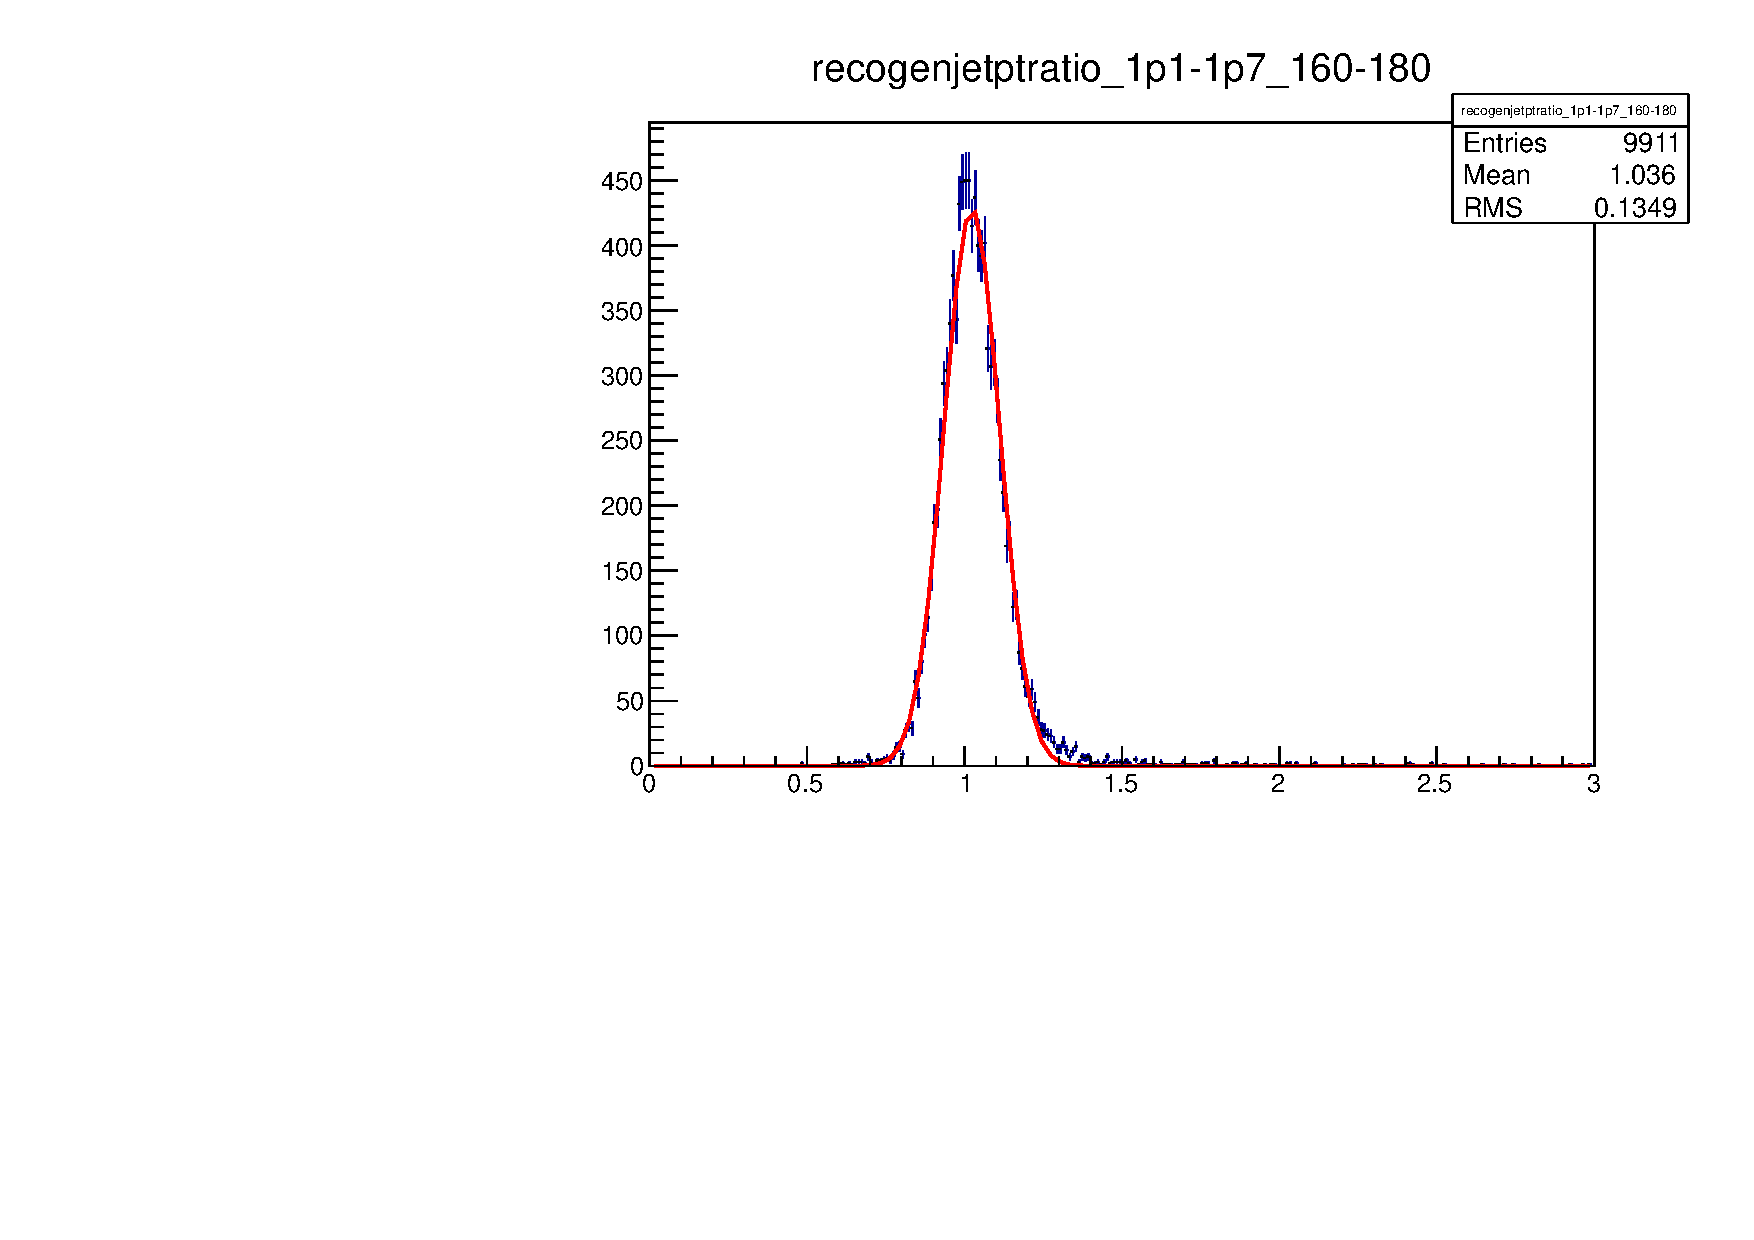
\includegraphics[width=1.1\textwidth]{TalkPics/jetres221013/recogenptratio1p1-1p7_160-180.pdf}
  \end{columns}
\end{frame}

\begin{frame}\label{lastframe}
  \frametitle{Plots}
  \begin{center}
  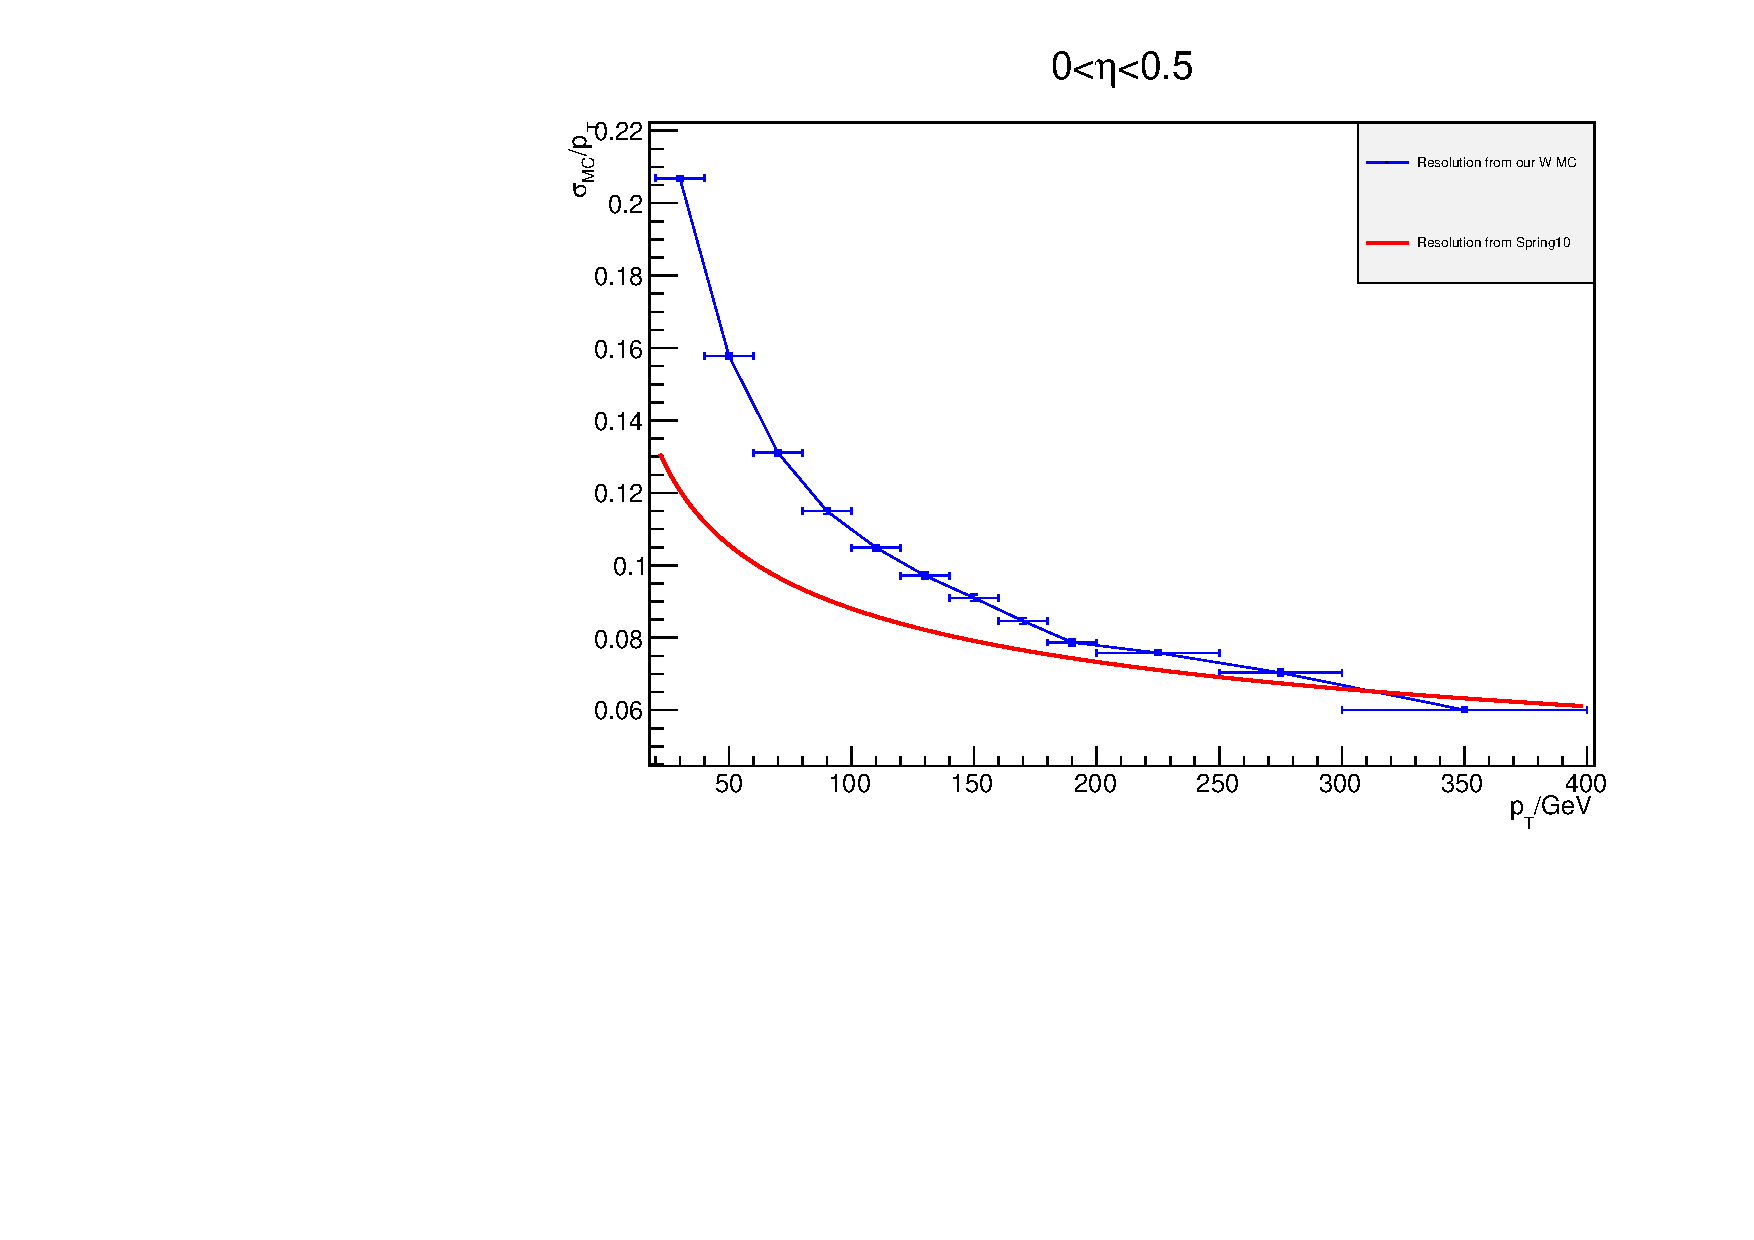
\includegraphics[width=.9\textwidth]{TalkPics/jetres221013/resforeta0p0-0p5.pdf}
  \end{center}
\end{frame}

\begin{frame}\label{lastframe}
  \frametitle{Plots}
  \begin{center}
  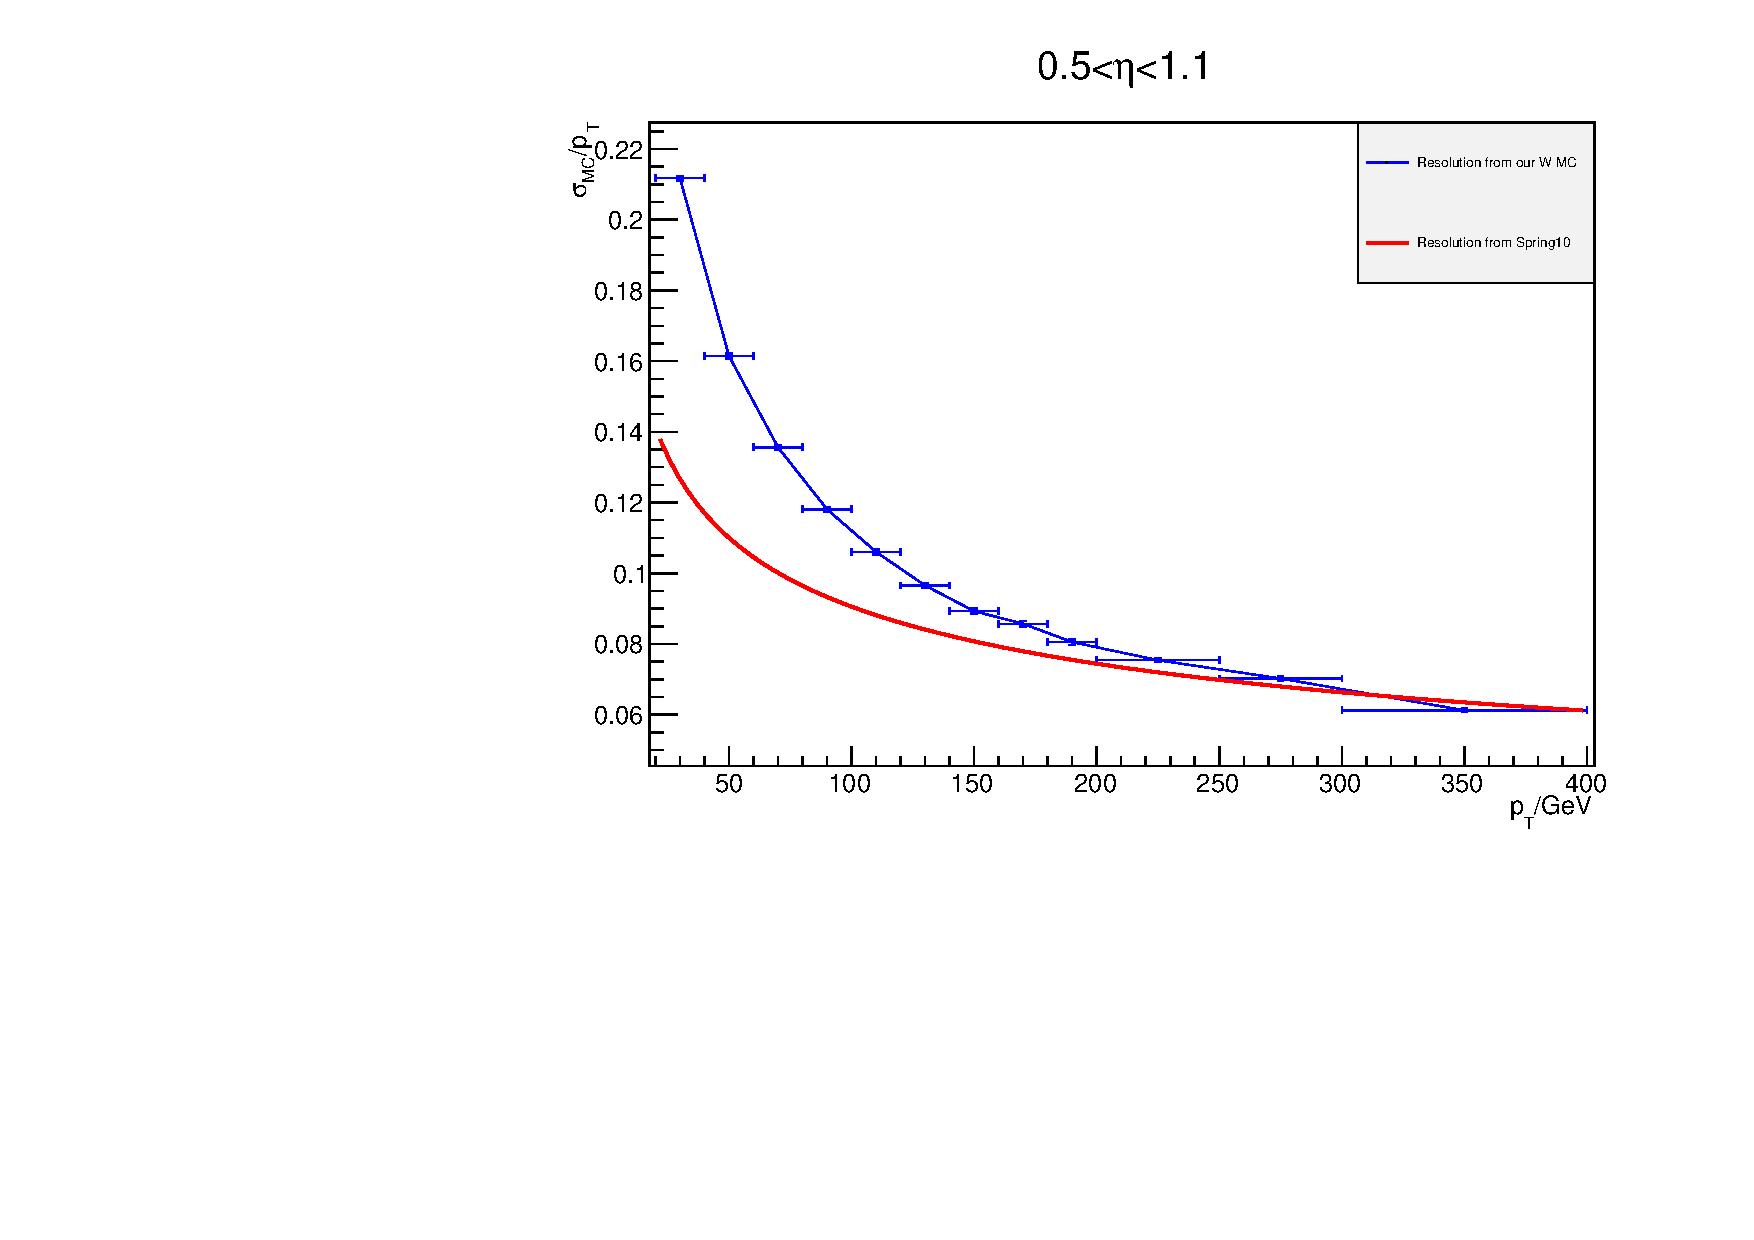
\includegraphics[width=.9\textwidth]{TalkPics/jetres221013/resforeta0p5-1p1.pdf}
  \end{center}
\end{frame}

\begin{frame}\label{lastframe}
  \frametitle{Plots}
  \begin{center}
  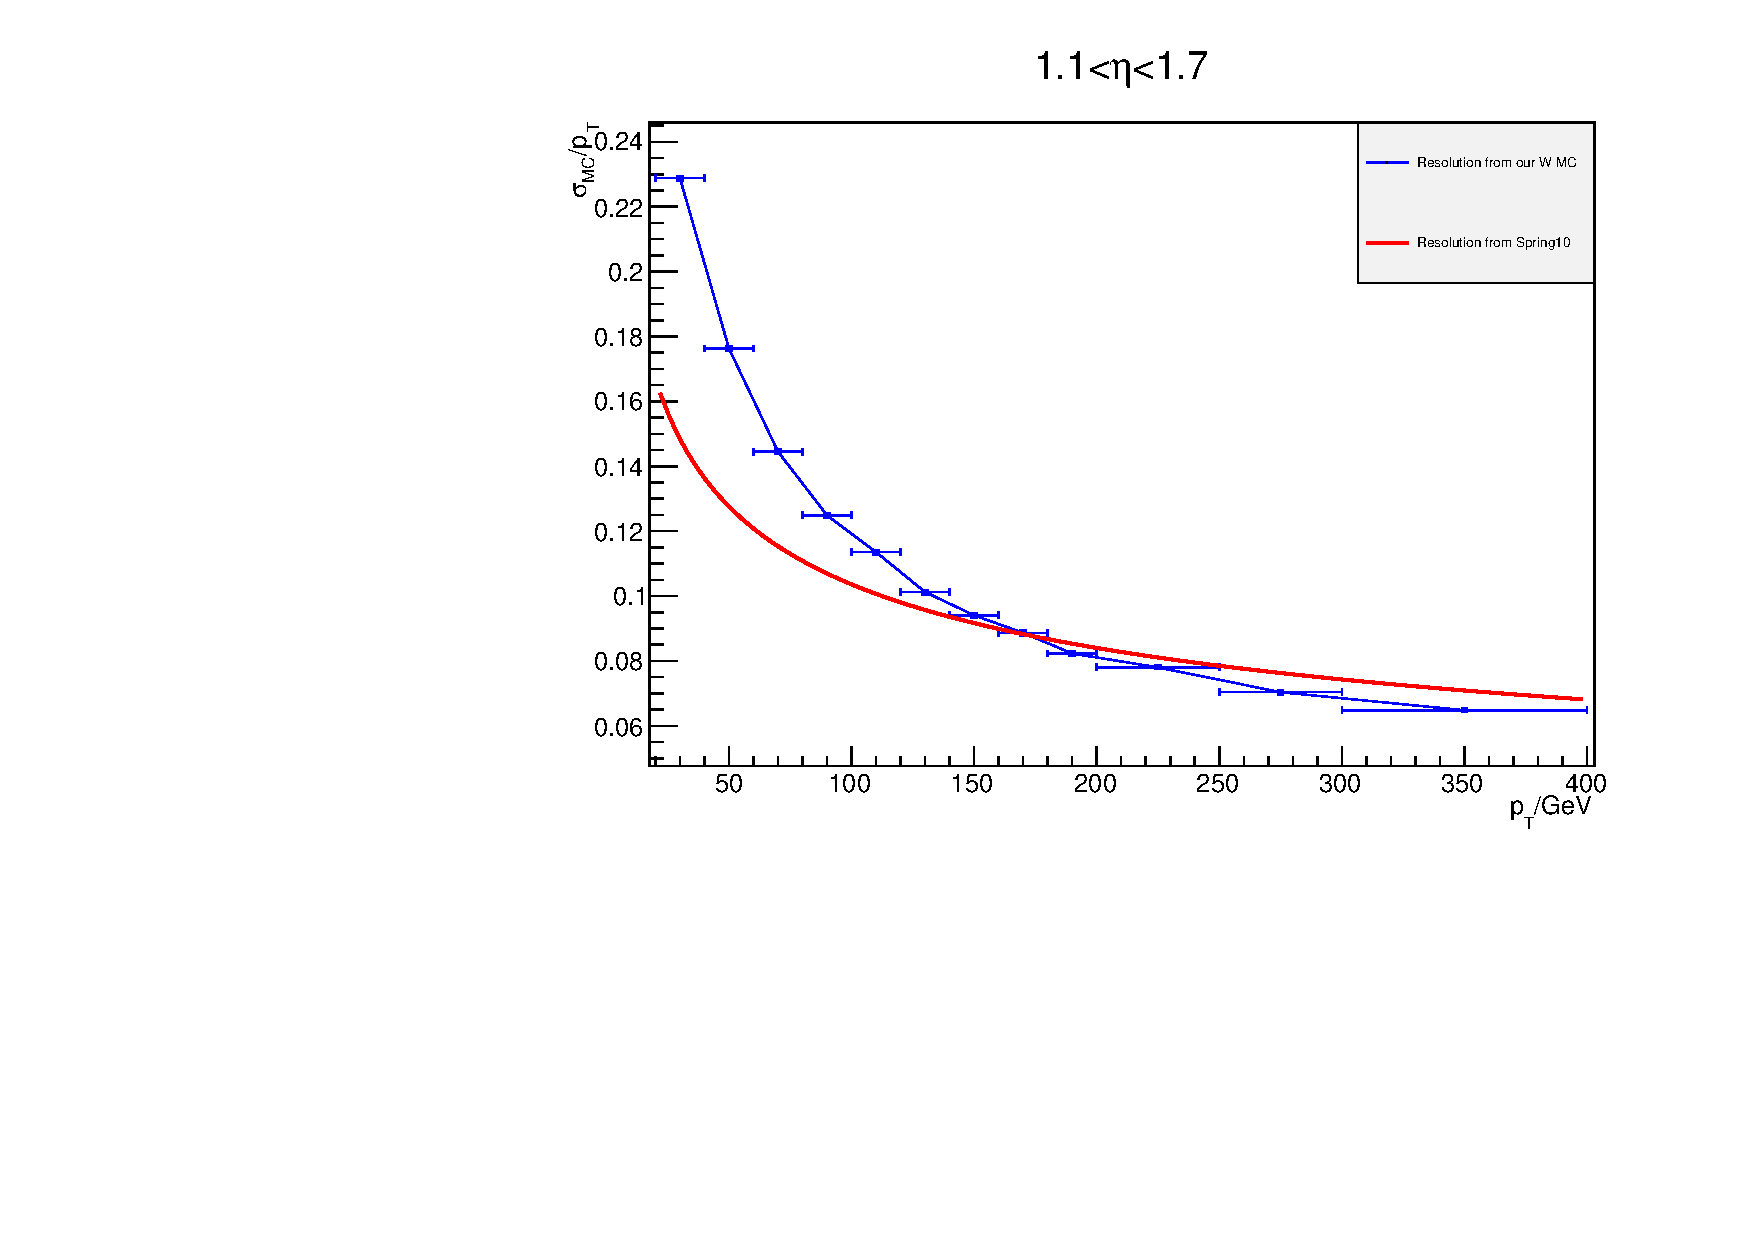
\includegraphics[width=.9\textwidth]{TalkPics/jetres221013/resforeta1p1-1p7.pdf}
  \end{center}
\end{frame}

\begin{frame}\label{lastframe}
  \frametitle{Plots}
  \begin{center}
  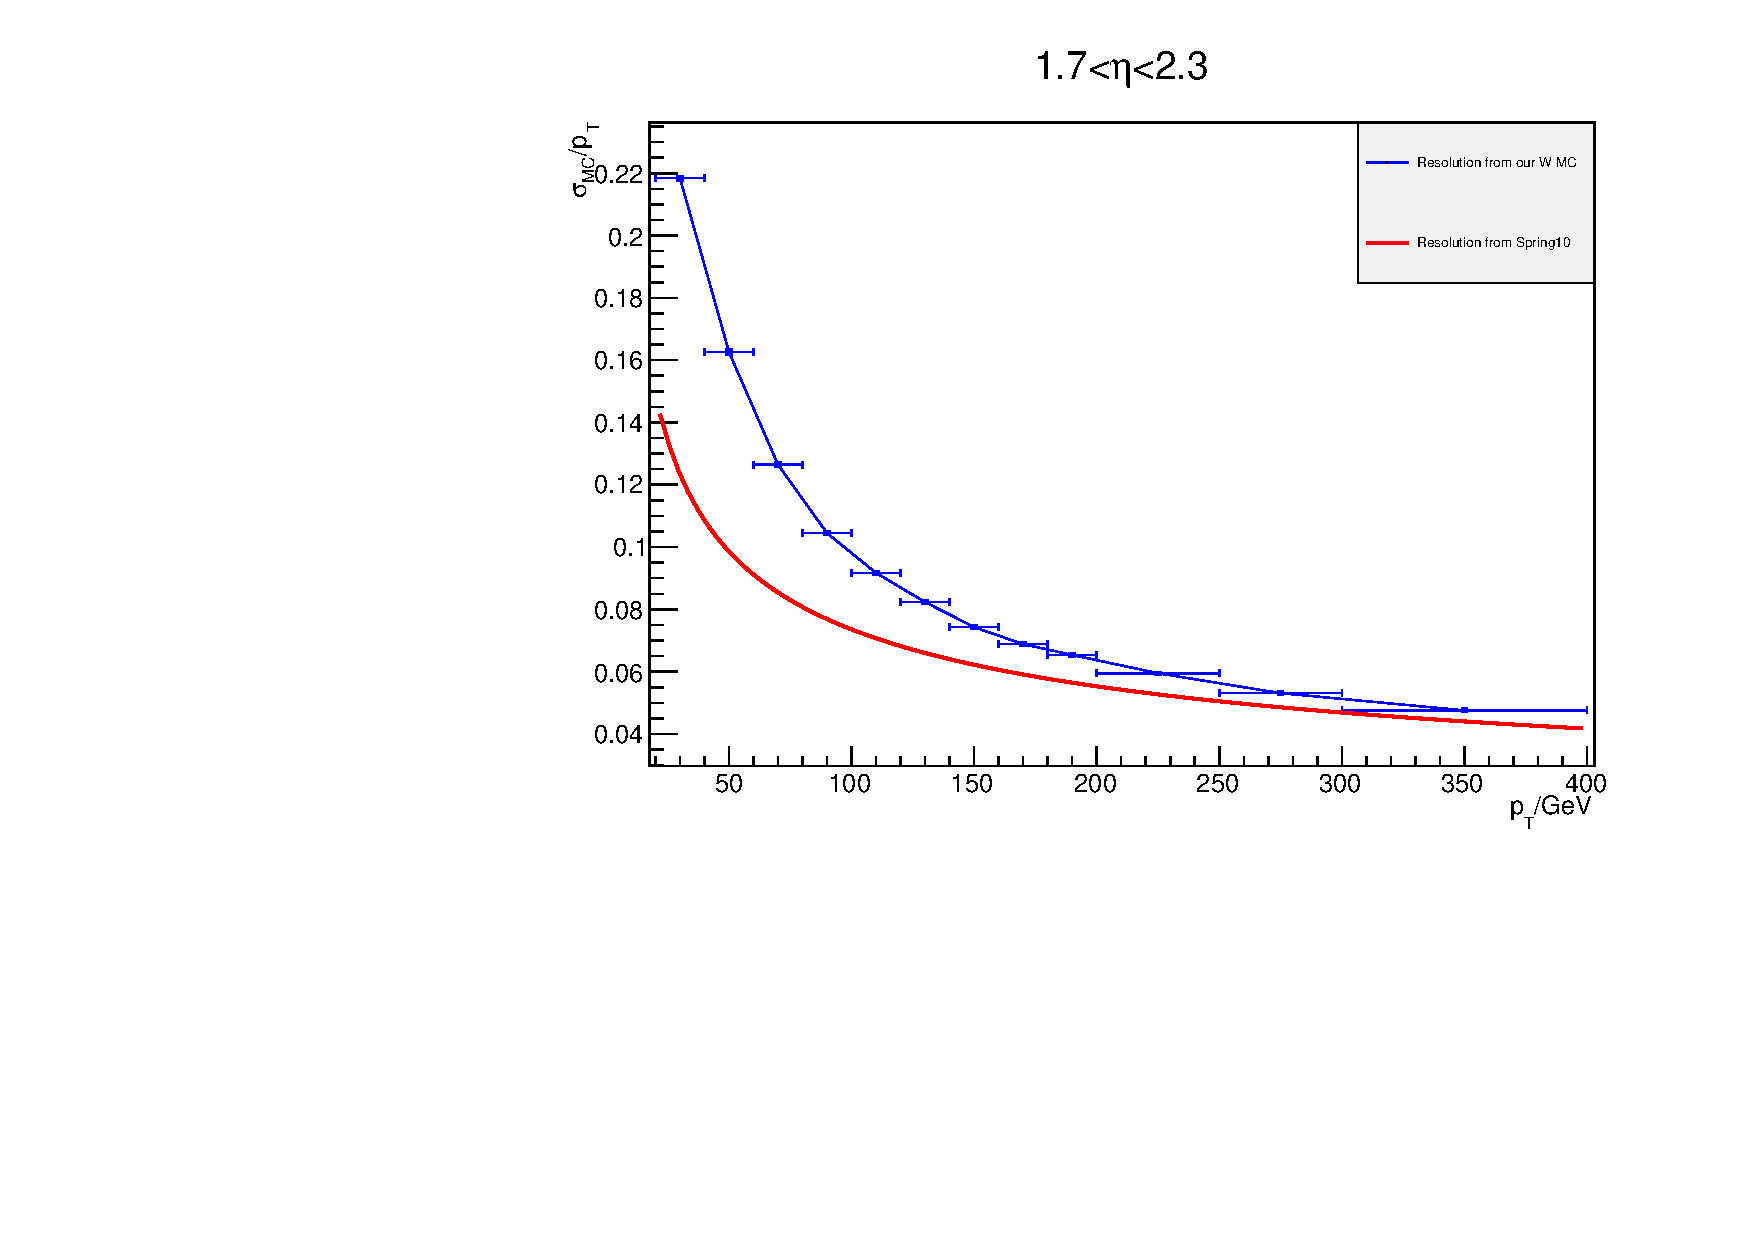
\includegraphics[width=.9\textwidth]{TalkPics/jetres221013/resforeta1p7-2p3.pdf}
  \end{center}
\end{frame}

\begin{frame}\label{lastframe}
  \frametitle{Plots}
  \begin{center}
  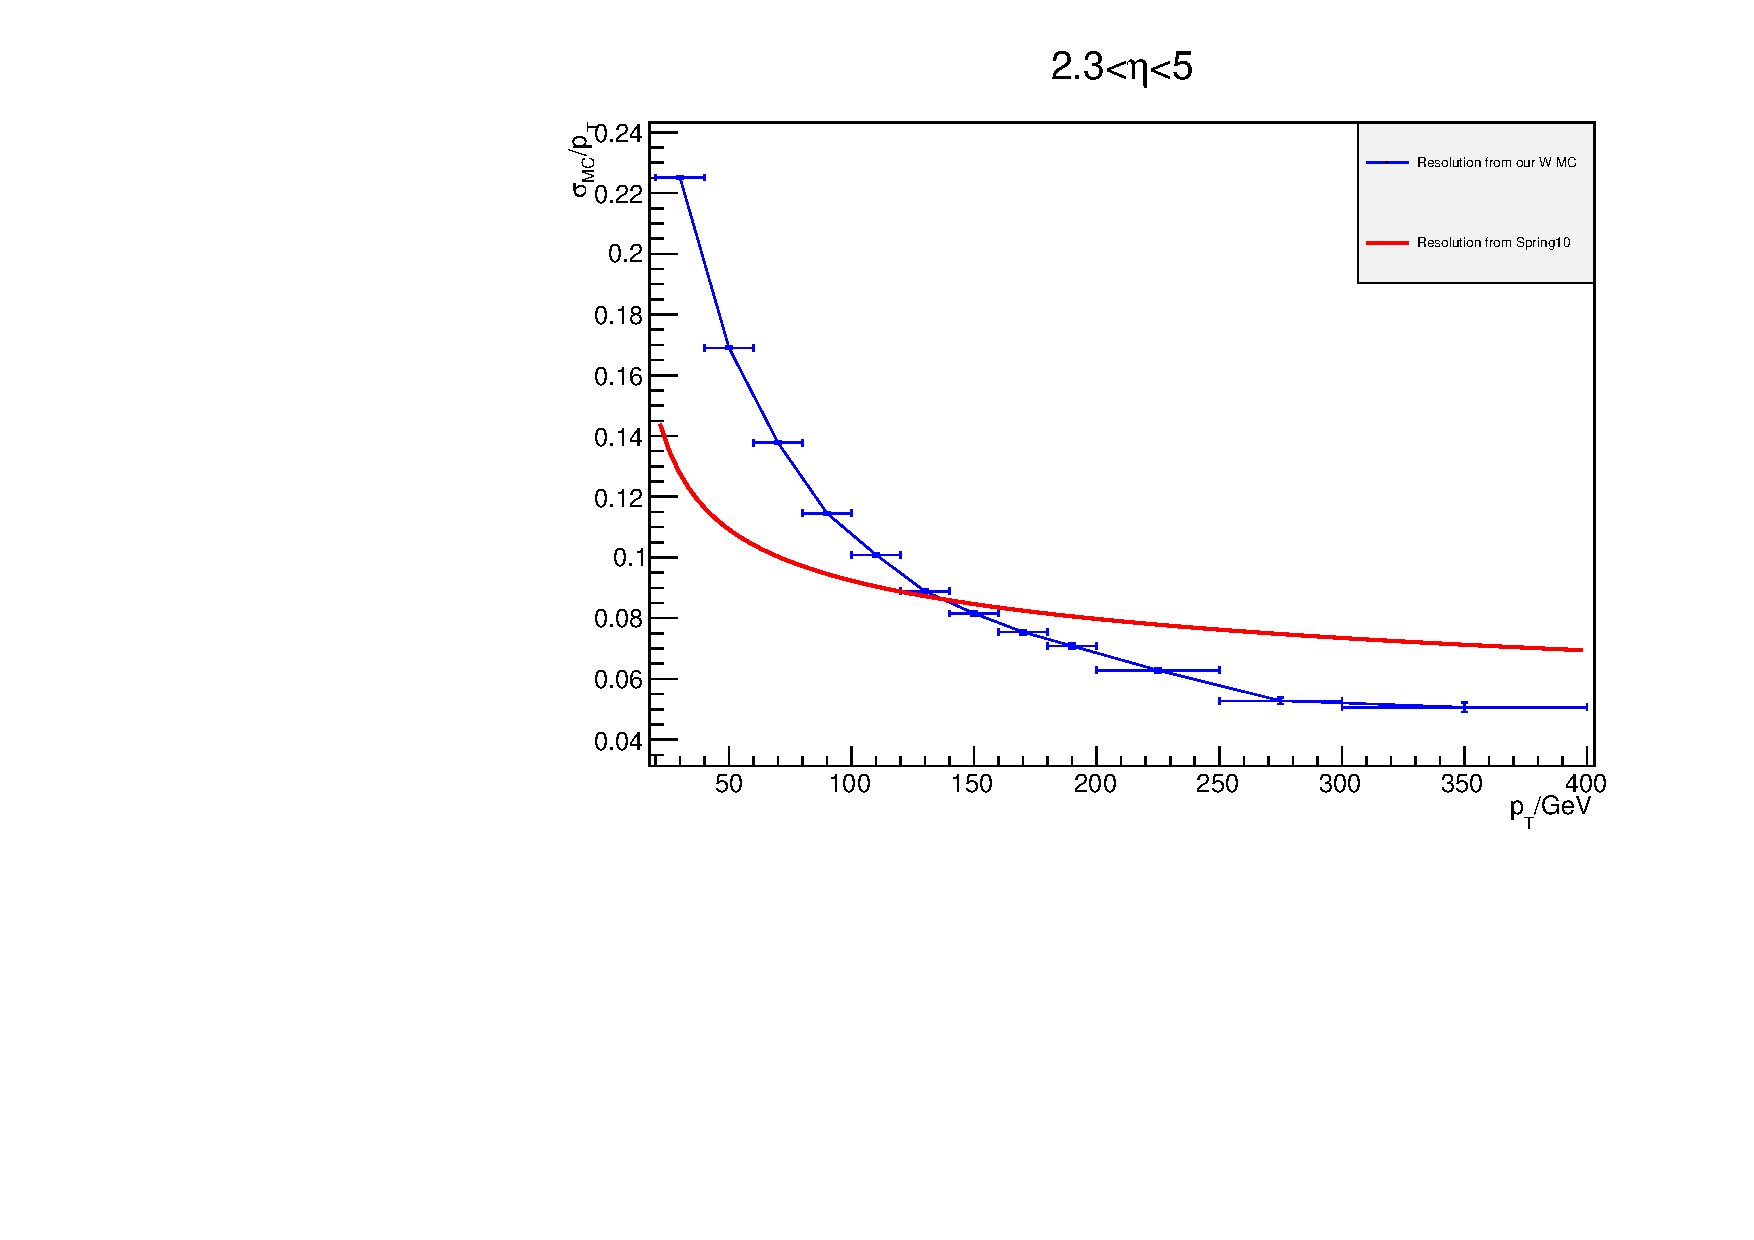
\includegraphics[width=.9\textwidth]{TalkPics/jetres221013/resforeta2p3-5p0.pdf}
  \end{center}
\end{frame}


\end{fmffile}
\end{document}
